\documentclass[aspectratio=169]{beamer}

\usepackage[T1]{fontenc}
\usepackage[utf8]{inputenc}
\usepackage{lmodern}

\usepackage{tikz}\usetikzlibrary{positioning}
\usepackage{xcolor}
\usepackage{hyperref}
\usepackage{listings}

\usetheme{metropolis}

\usepackage{FiraSans}

\newcommand<>{\cul}[2][red]{
  \fontdimen8\textfont3=0.75pt
  \alt#3
      {\color{#1}\underline{{\color{black}#2}}\color{black}}
      {\transparent{0.0}\underline{{\transparent{1.0}#2}}\transparent{1.0}}
}

\title{Callgrind \& Kcachegrind}
\author{Jiří Klepl}
\date{}
\begin{document}
\maketitle

\begin{frame}{Profiling a proč profilovat \small{(link na konci prezentace)}}
  \begin{quote}
    With application development, a common step is to improve runtime performance. To not waste time on optimizing functions which are rarely used, one needs to know in which parts of the program most of the time is spent.

    This is done with a technique called profiling. The program is run under control of a profiling tool, which gives the time distribution of executed functions in the run. After examination of the program's profile, it should be clear if and where optimization is useful. Afterwards, one should verify any runtime changes by another profile run. [\ref{manual2}]
  \end{quote}
\end{frame}

\begin{frame}{Callgrind}
  \begin{itemize}
    \item Profiler ve \textbf{valgrindovém} simulovaném prostředí
    \begin{itemize}
      \item valgrind disassembluje binárky a sestavuje podle daného nástroje (zde s instrumentací)
      \item základní nástroj valgrindu je memcheck, který kontroluje leaky a chybné přístupy
    \end{itemize}
    \item Analyzuje \textbf{call-graph}; ale také i instrukce uvnitř funkcí a branch predikce, simulace cache (podle optionů)
    \item Odvozen z nástroje \textbf{cachegrind}, stejný formát výstupu; obojí lze zobrazit v \textbf{kcachegrind} (nebo \textbf{qcachegrind})
  \end{itemize}
\end{frame}

\begin{frame}[fragile]{Srovnání s konvenčnějším profilingem (e.g. gprof)}

  {\color{green} \textbf{Výhody}}

  \begin{itemize}
    \item Pohodlnost (stačí normální \textit{release} binárka s debug flagy - není nutno compilovat se speciálními optiony (u gprof \texttt{-pg}))
    \item Přesnost měření a nezávislost na aktuálním zatížení stroje
    \item Profiling neovlivňuje aplikaci (to je u běžné instrumentace velký problém)
    \item Profilují se i dynamicky linkované knihovny (= profiler vidí vše)
    \item Lze za běhu ovládat (nemusíme trávit staletí profilingem startupu, když nás zajímá jen jedna funkce)
  \end{itemize}

  {\color{red} \textbf{Nevýhody}}

  \begin{itemize}
    \item Pomalost (valgrind uvádí 50x slowdown)
    \item Limitovaná podpora méně mainstream architektur (u AMD64 není problém)
  \end{itemize}
\end{frame}

\begin{frame}[fragile]{Základní použití callgrindu}
  \begin{lstlisting}[language=sh]
valgrind --tool=callgrind [options] your-program [arguments]
  \end{lstlisting}
  {\color{blue} \lstinline{your-program} by měl mít debug flagy a narozdíl od debuggingu by měl být optimalizován}

  \textbf{Základní optiony}

  \begin{itemize}
    \item \lstinline{--dump-instr=yes}: zanalyzuje machine code
    \item \lstinline{--collect-jumps=yes}: zanalyzuje branching
    \item \lstinline{--cache-sim=yes}: simulace cache
  \end{itemize}

  Výstup je v souboru: \texttt{callgrind.out.pid.part-threadID} (thready!)
\end{frame}

\begin{frame}{Kcachegrind (qcachegrind)}
  \begin{itemize}
    \item GUI procházení výstupu nástrojů \textbf{cachegrind} a \textbf{callgrind}
    \item Velice intuitivní a feature-rich s procházením kódu (a nastavitelný)
  \end{itemize}
  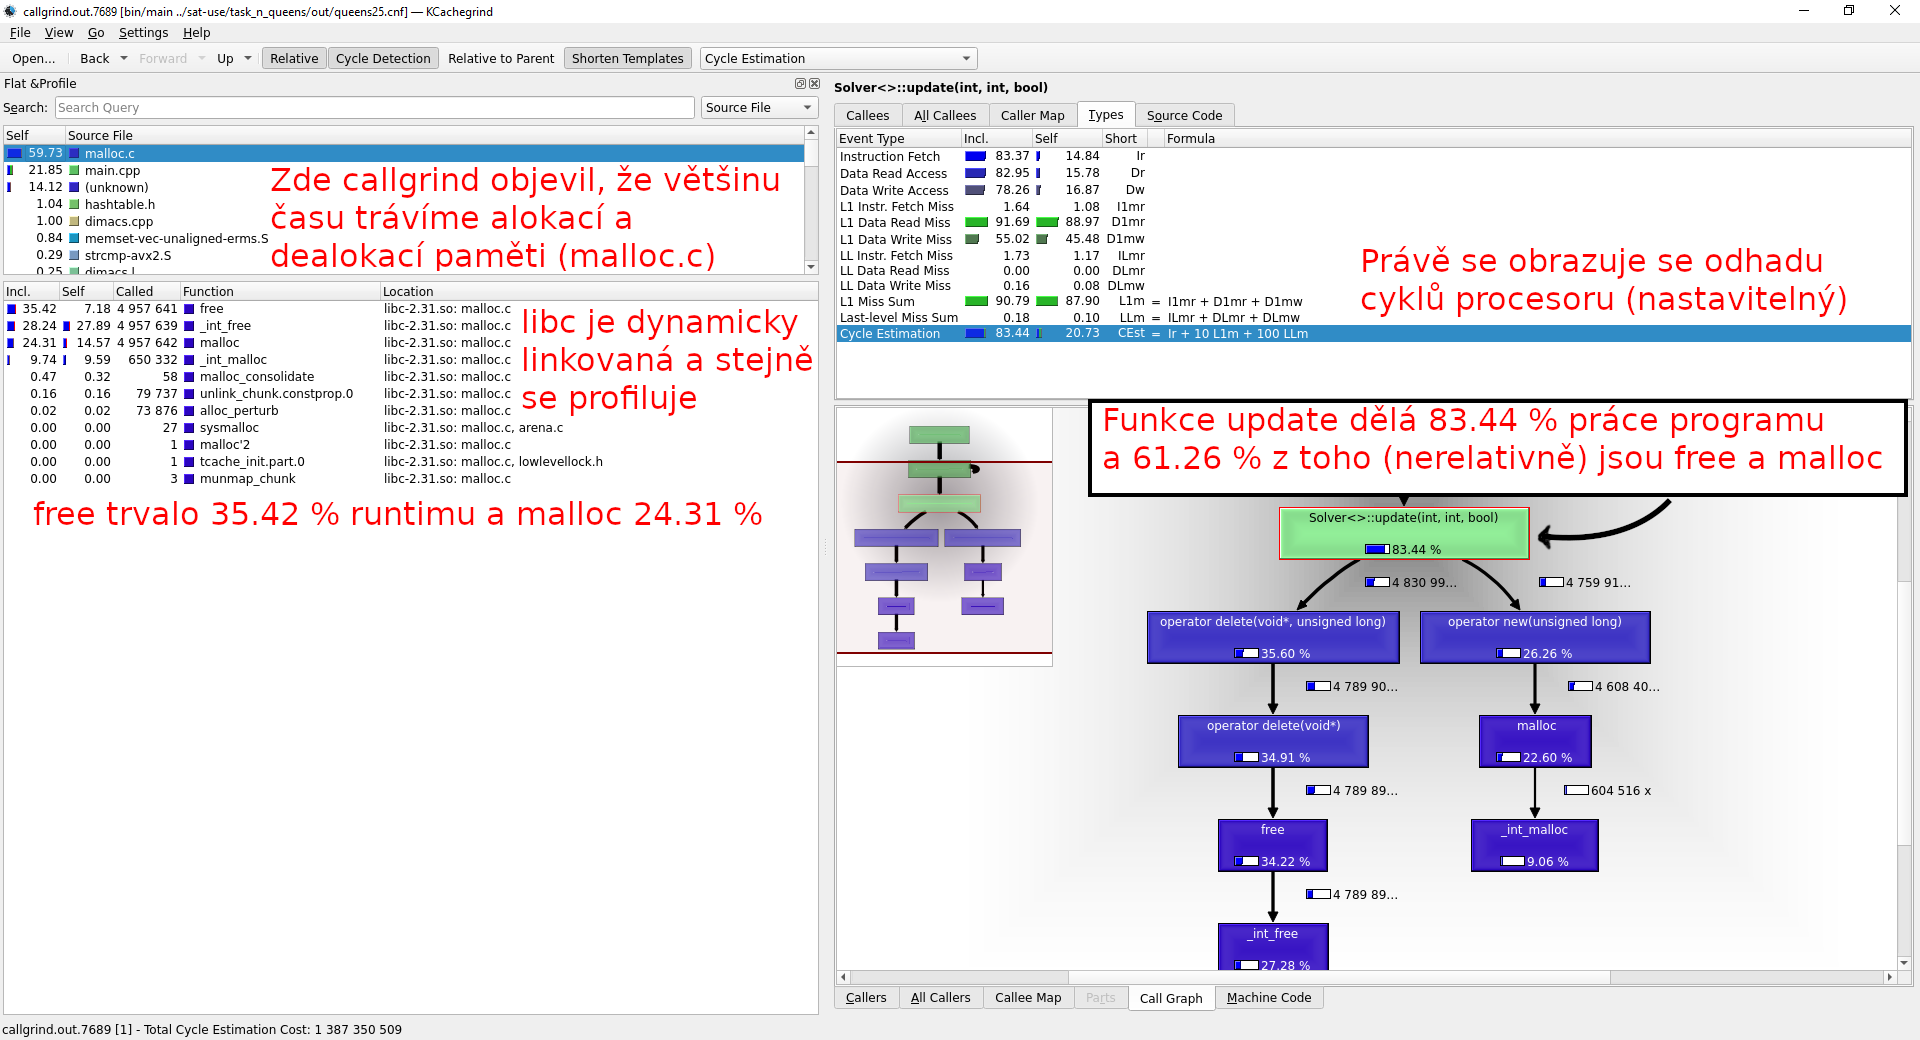
\includegraphics[width=.9 \linewidth]{callgrind.png}
\end{frame}

\begin{frame}[fragile]{Demonstrace}
  Ve složce \texttt{/callgrind} uvnitř tohoto repa (link: \href{https://github.com/jiriklepl/NSWI126/tree/master/callgrind}{NSWI126/callgrind})
  \begin{lstlisting}[language=sh]
    cd ex1
    kcachegrind callgrind.out.7689
  \end{lstlisting}
  \begin{lstlisting}[language=sh]
    cd ex2
    kcachegrind callgrind.out.7787
  \end{lstlisting}
\end{frame}

\begin{frame}[fragile]{Více informací}
  \begin{enumerate}
    \item \href{https://valgrind.org/docs/manual/cl-manual.html}{https://valgrind.org/docs/manual/cl-manual.html}
    \item \label{manual2} \href{https://www.cs.cmu.edu/afs/cs.cmu.edu/project/cmt-40/Nice/RuleRefinement/bin/valgrind-3.2.0/docs/html/cl-manual.html}{https://www.cs.cmu.edu/afs/cs.cmu.edu/.../cl-manual.html}
  \end{enumerate}
\end{frame}

\begin{frame}[plain]
  \centering
  {\Large\bfseries Díky za pozornost!}
\end{frame}

\end{document}
